\chapter{T\'ecnicas de selecci\'on de pivotes}\label{anexo.A}
A continuaci\'on incluimos las graficas correspondientes al efecto de las t\'ecnicas de selecci\'on para cada una de las bases de datos que utilizamos.\\

\begin{figure}[h!]
\centering
{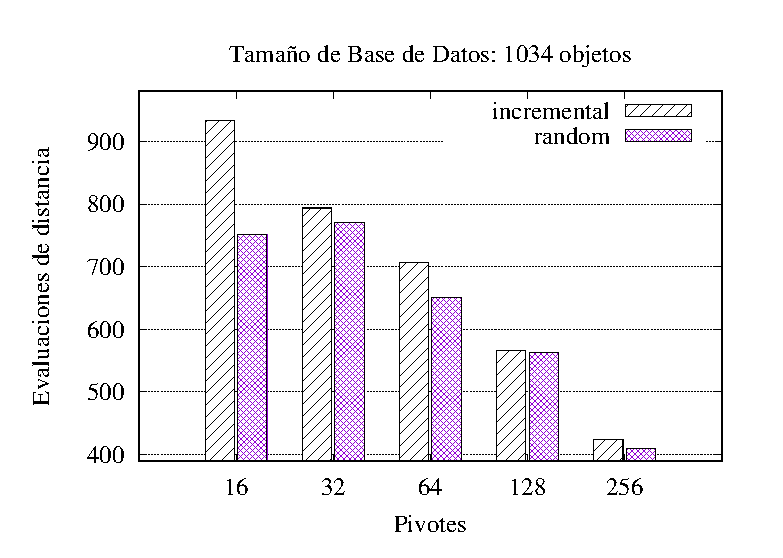
\includegraphics[width=71.5mm]{imagenes/random_vs_incremental/g1_1034.eps}}
{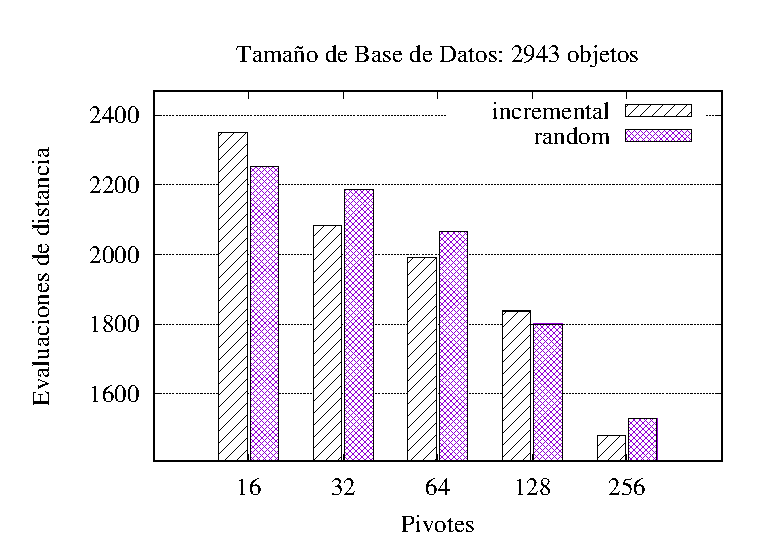
\includegraphics[width=71.5mm]{imagenes/random_vs_incremental/g1_2943.eps}}
{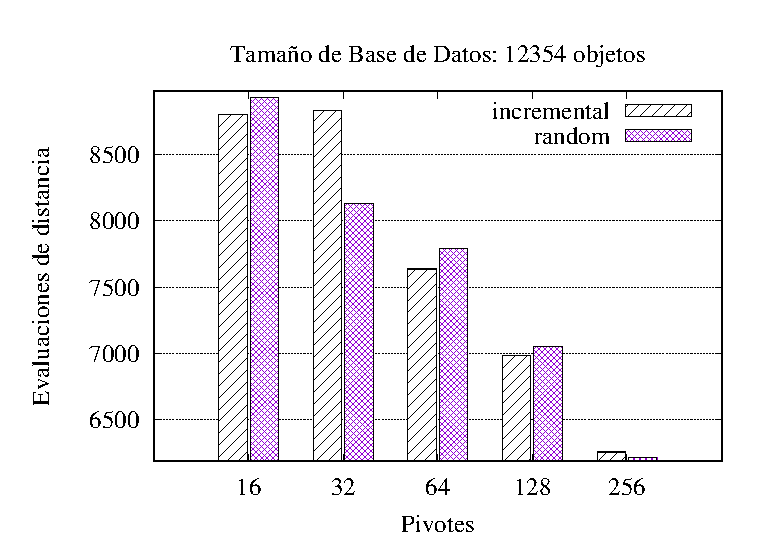
\includegraphics[width=71.5mm]{imagenes/random_vs_incremental/g1_12354.eps}}
{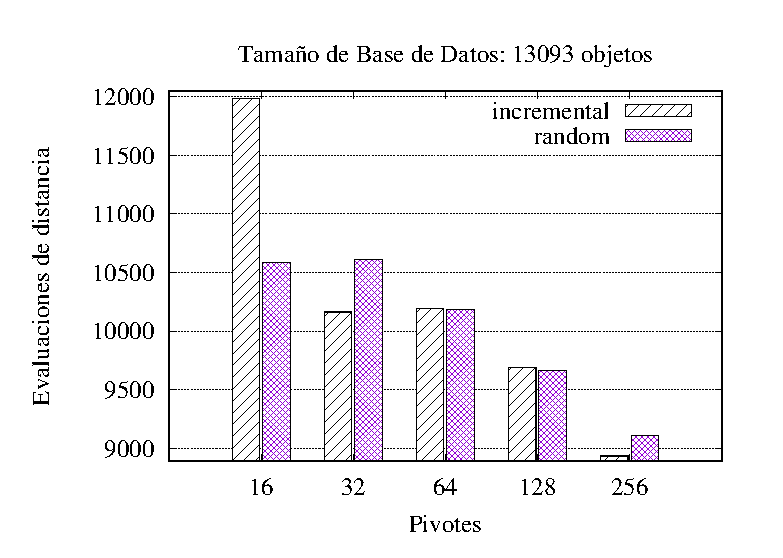
\includegraphics[width=71.5mm]{imagenes/random_vs_incremental/g1_13093.eps}}
\caption{\small Grupo 1 - Efecto de las t\'ecnicas de selecci\'on de pivotes random vs incremental respecto de evaluaciones de distancia.}
\end{figure}

\begin{figure}[h!]
\centering
{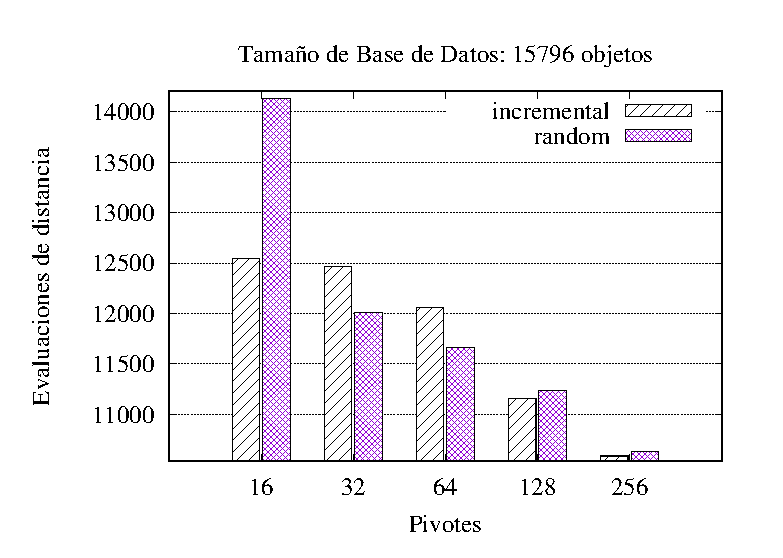
\includegraphics[width=71.5mm]{imagenes/random_vs_incremental/g1_15796.eps}}
{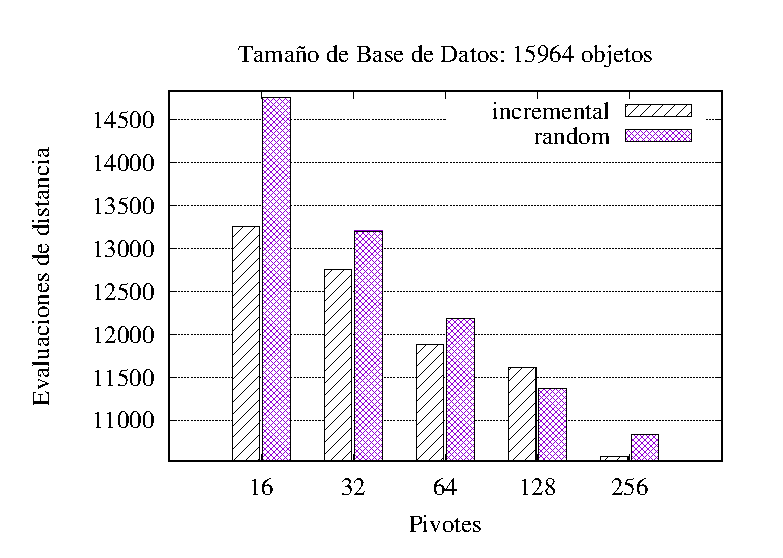
\includegraphics[width=71.5mm]{imagenes/random_vs_incremental/g1_15964.eps}}
\caption{\small Grupo 1 - Efecto de las t\'ecnicas de selecci\'on de pivotes random vs incremental respecto de evaluaciones de distancia.}
\end{figure}

\begin{figure}[h!]
\centering
{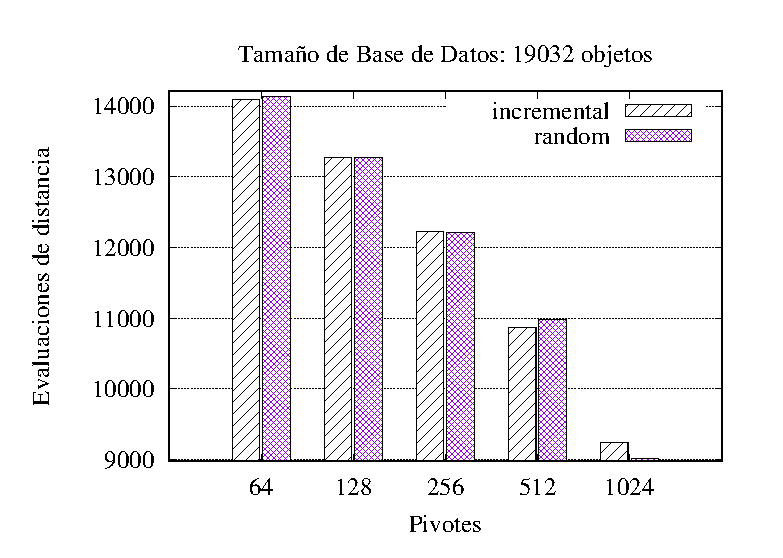
\includegraphics[width=71.5mm]{imagenes/random_vs_incremental/g2_19032.eps}}
{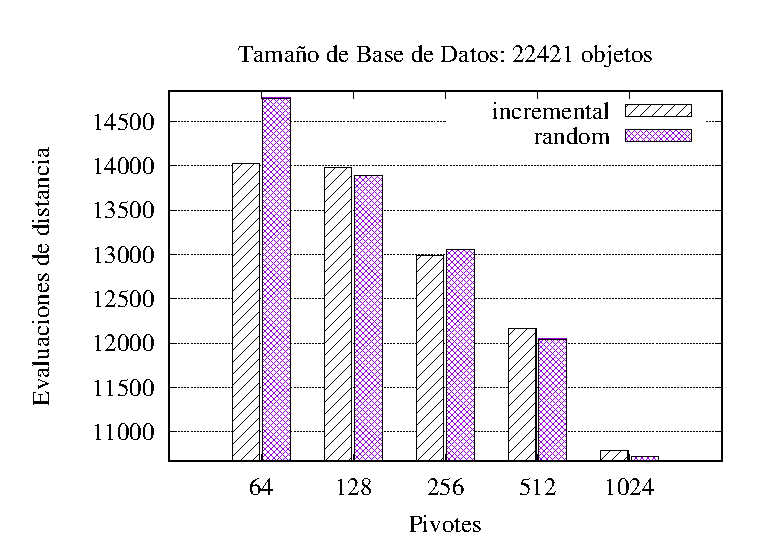
\includegraphics[width=71.5mm]{imagenes/random_vs_incremental/g2_22421.eps}}
{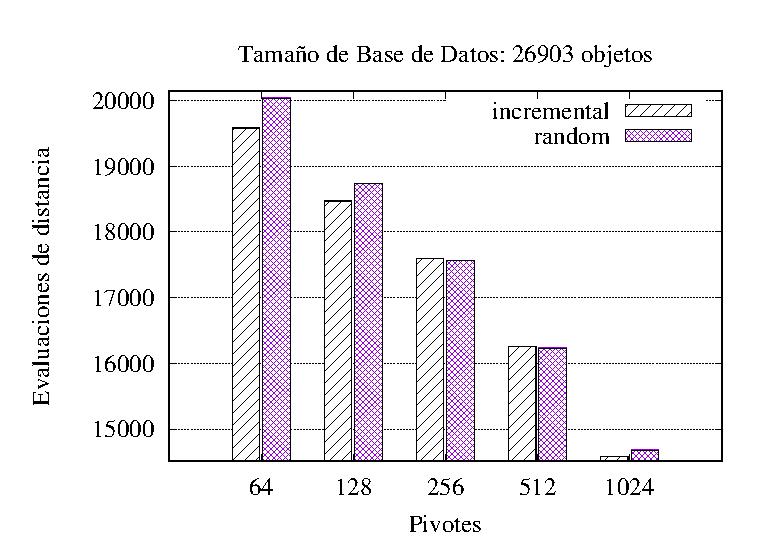
\includegraphics[width=71.5mm]{imagenes/random_vs_incremental/g2_26903.eps}}
{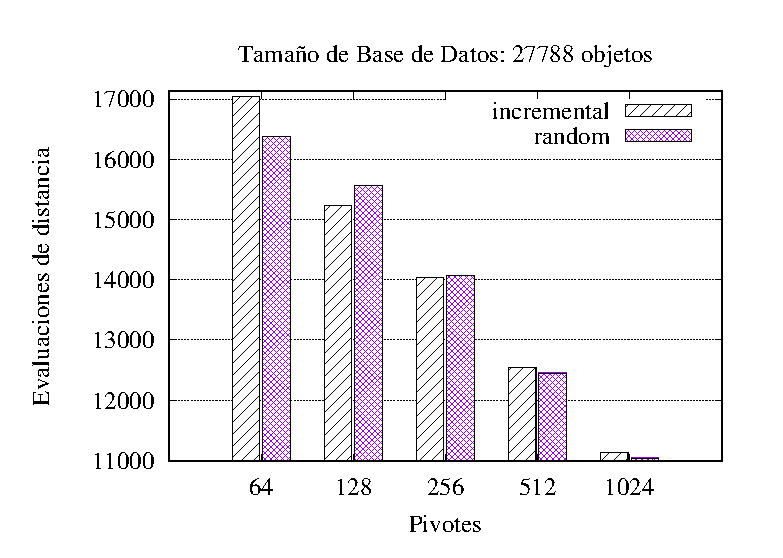
\includegraphics[width=71.5mm]{imagenes/random_vs_incremental/g2_27788.eps}}
\caption{\small Grupo 2 - Efecto de las t\'ecnicas de selecci\'on de pivotes random vs incremental respecto de evaluaciones de distancia.}
\end{figure}
\begin{figure}[h!]
\centering
{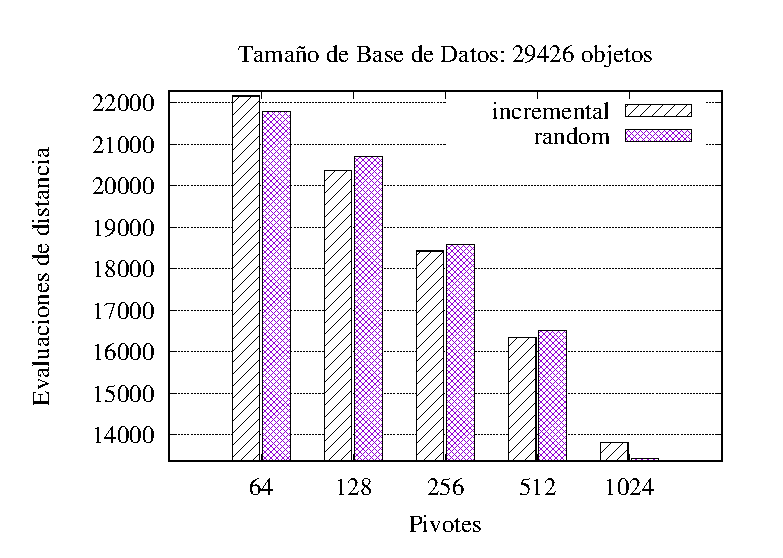
\includegraphics[width=71.5mm]{imagenes/random_vs_incremental/g2_29426.eps}}
{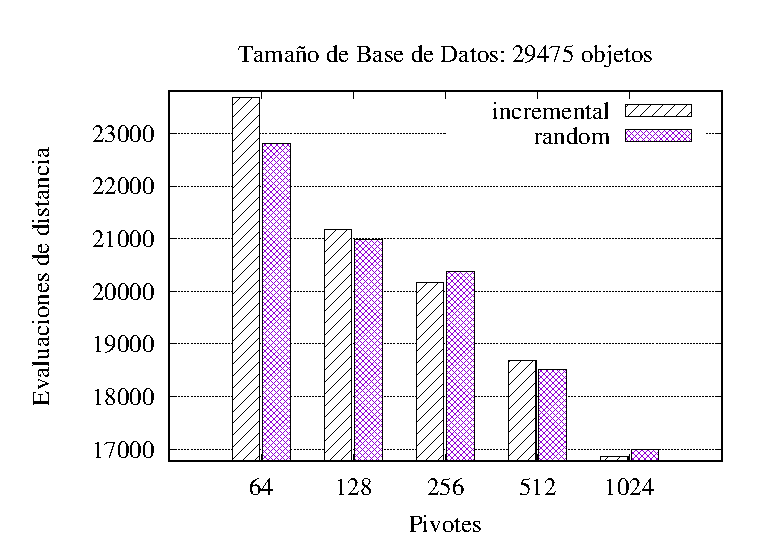
\includegraphics[width=71.5mm]{imagenes/random_vs_incremental/g2_29475.eps}}
{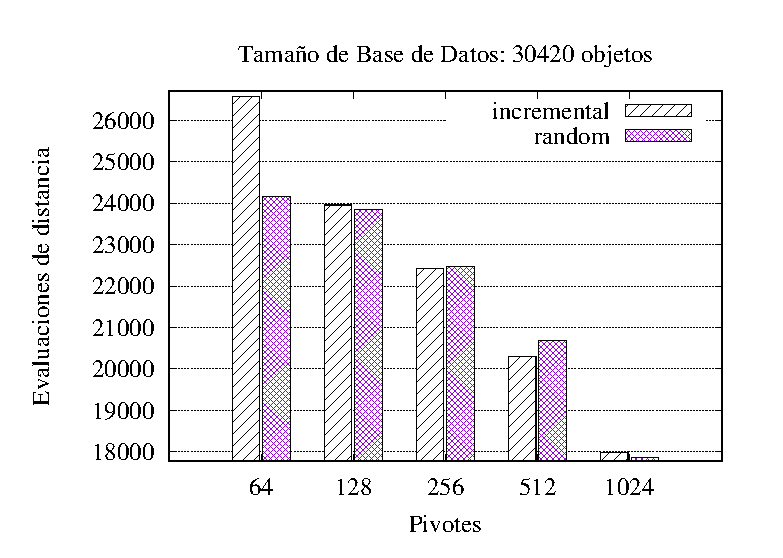
\includegraphics[width=71.5mm]{imagenes/random_vs_incremental/g2_30420.eps}}
{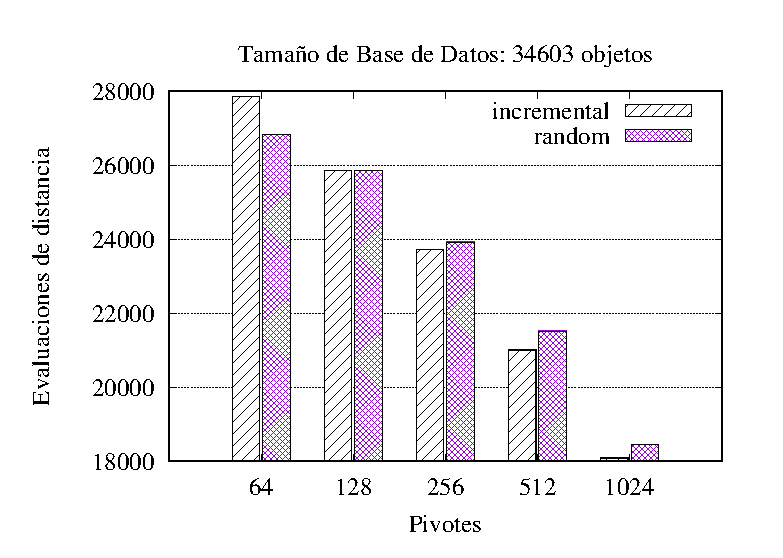
\includegraphics[width=71.5mm]{imagenes/random_vs_incremental/g2_34603.eps}}
{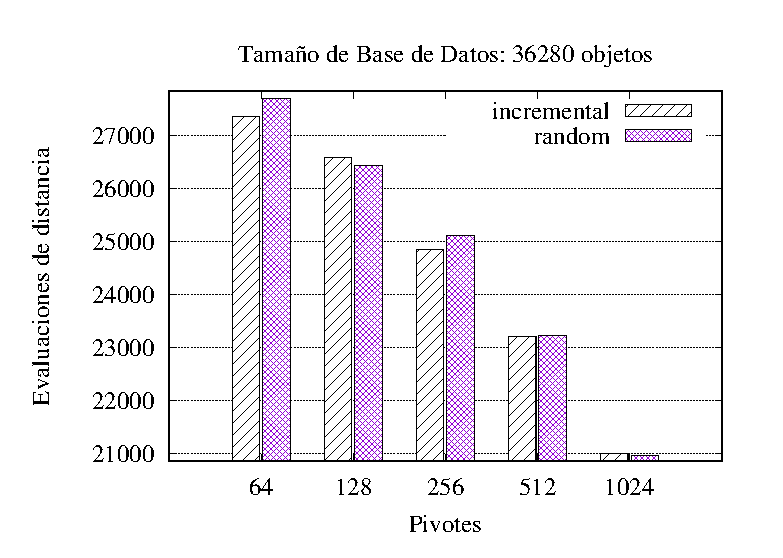
\includegraphics[width=71.5mm]{imagenes/random_vs_incremental/g2_36280.eps}}
{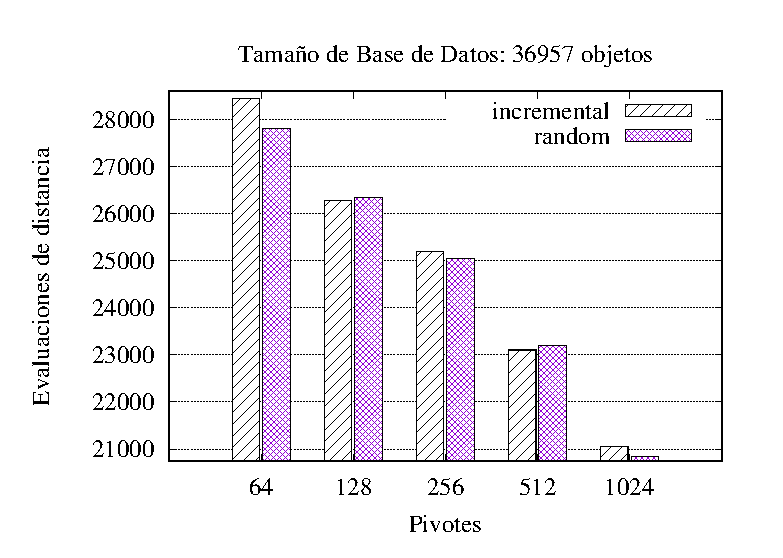
\includegraphics[width=71.5mm]{imagenes/random_vs_incremental/g2_36957.eps}}
{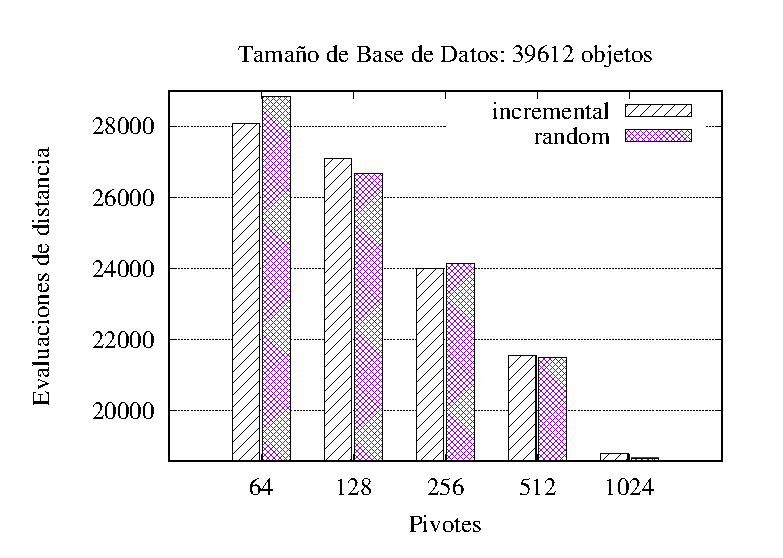
\includegraphics[width=71.5mm]{imagenes/random_vs_incremental/g2_39612.eps}}
{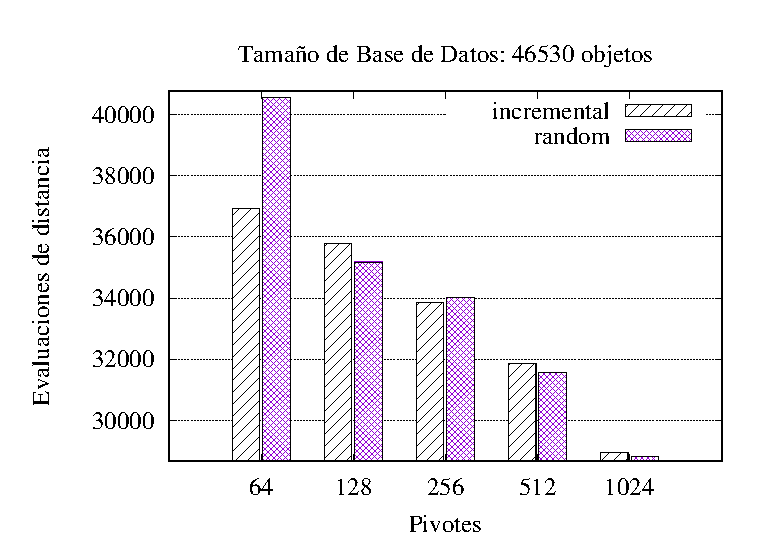
\includegraphics[width=71.5mm]{imagenes/random_vs_incremental/g2_46530.eps}}
\caption{\small Grupo 2 - Efecto de las t\'ecnicas de selecci\'on de pivotes random vs incremental respecto de evaluaciones de distancia.}
\end{figure}


\begin{figure}[h!]
\centering
{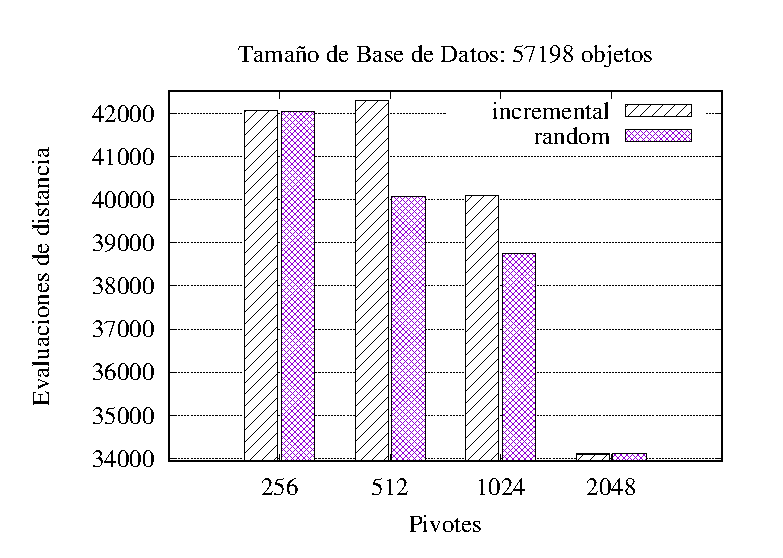
\includegraphics[width=71.5mm]{imagenes/random_vs_incremental/g3_57198.eps}}
{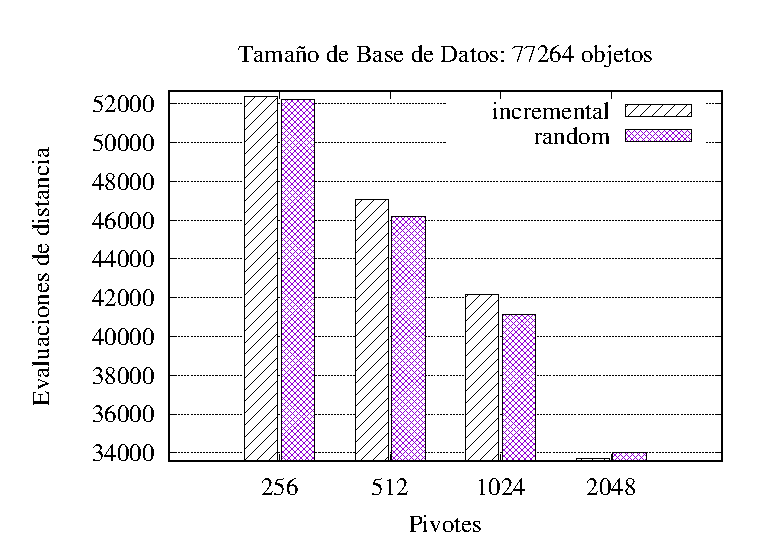
\includegraphics[width=71.5mm]{imagenes/random_vs_incremental/g3_77264.eps}}
{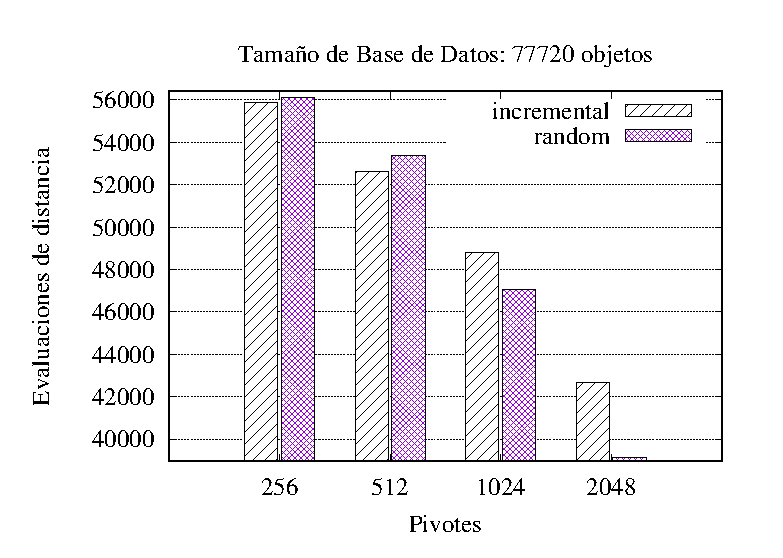
\includegraphics[width=71.5mm]{imagenes/random_vs_incremental/g3_77720.eps}}
{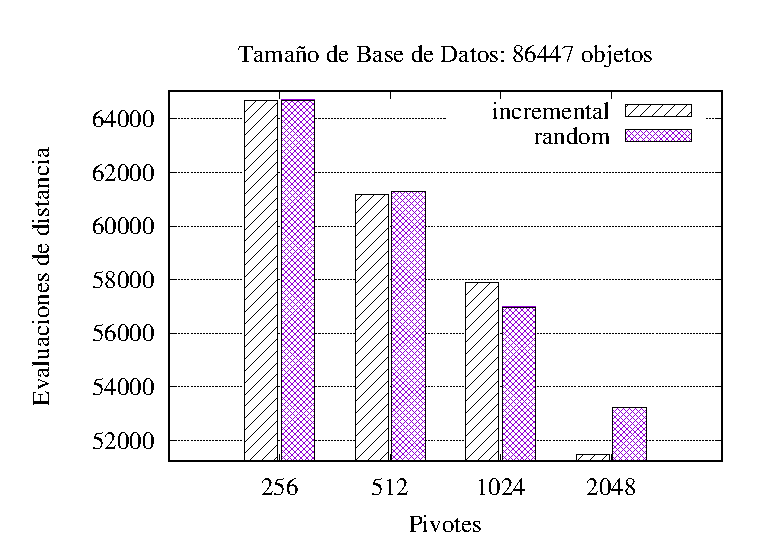
\includegraphics[width=71.5mm]{imagenes/random_vs_incremental/g3_86447.eps}}
{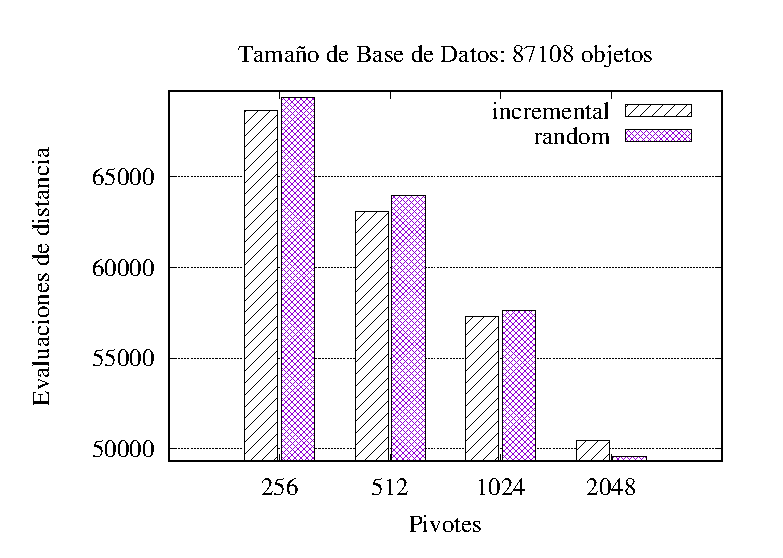
\includegraphics[width=71.5mm]{imagenes/random_vs_incremental/g3_87108.eps}}
{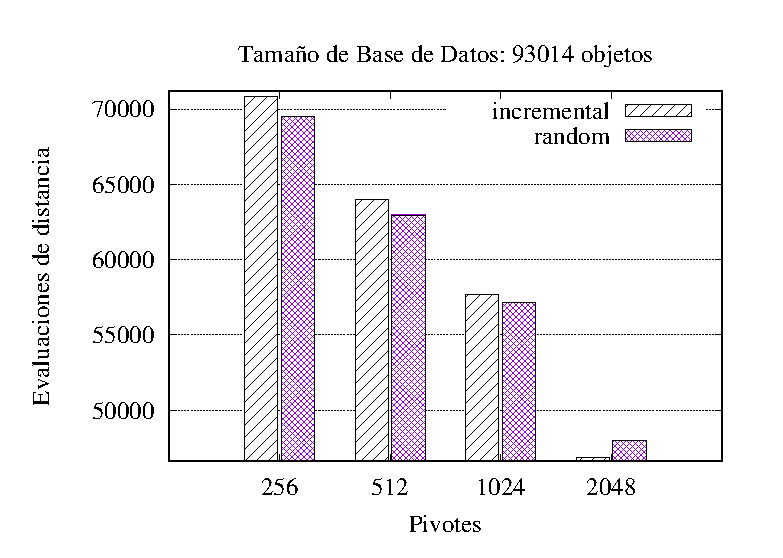
\includegraphics[width=71.5mm]{imagenes/random_vs_incremental/g3_93014.eps}}
{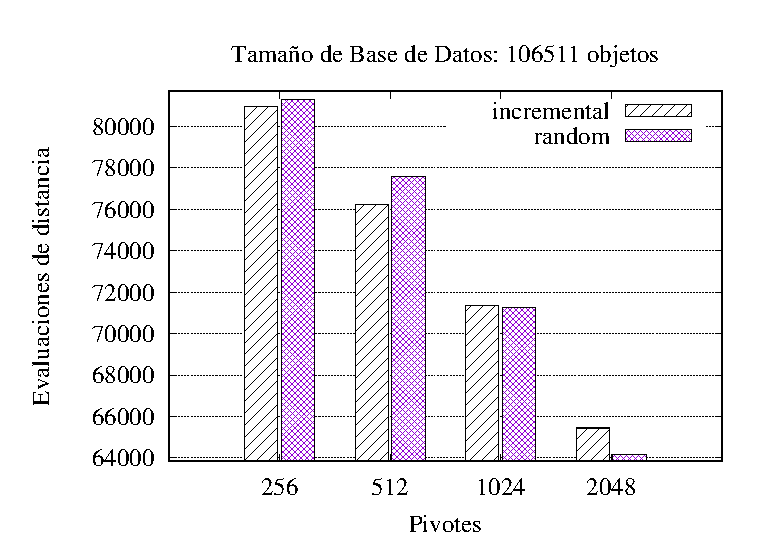
\includegraphics[width=71.5mm]{imagenes/random_vs_incremental/g3_106511.eps}}
{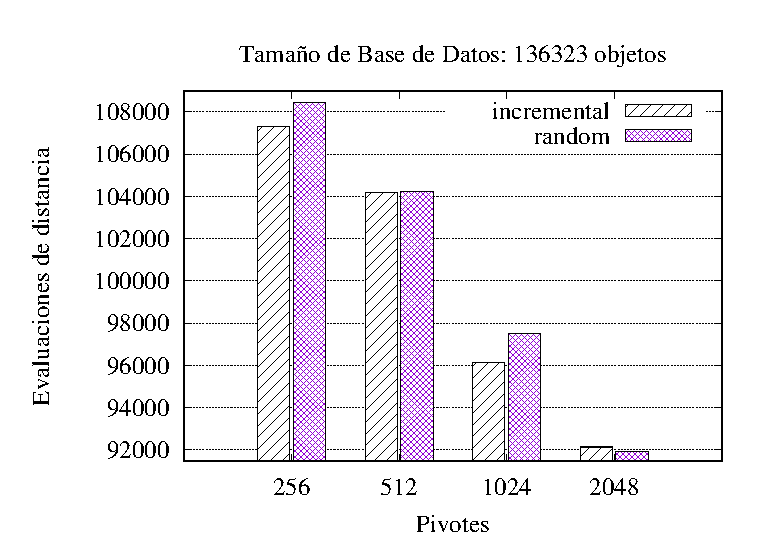
\includegraphics[width=71.5mm]{imagenes/random_vs_incremental/g3_136323.eps}}
\caption{\small Grupo 3 - Efecto de las t\'ecnicas de selecci\'on de pivotes random vs incremental respecto de evaluaciones de distancia.}
\end{figure}

\begin{figure}[h!]
\centering
{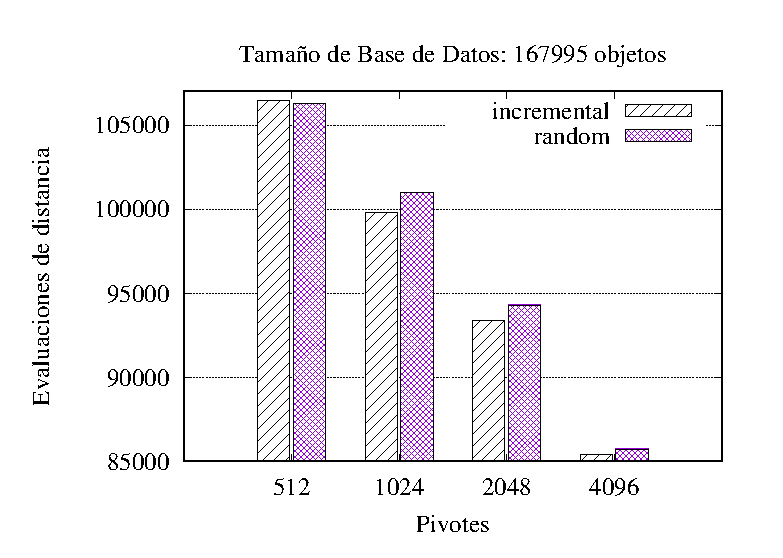
\includegraphics[width=71.5mm]{imagenes/random_vs_incremental/g4_167995.eps}}
{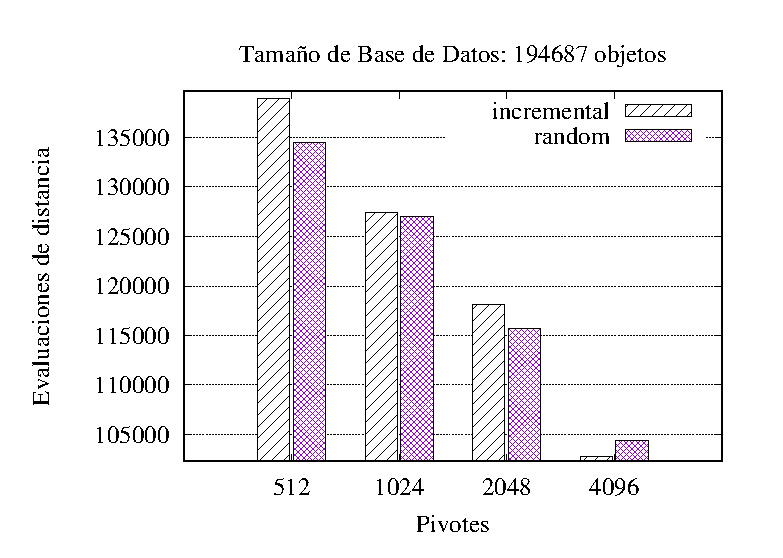
\includegraphics[width=71.5mm]{imagenes/random_vs_incremental/g4_194687.eps}}
{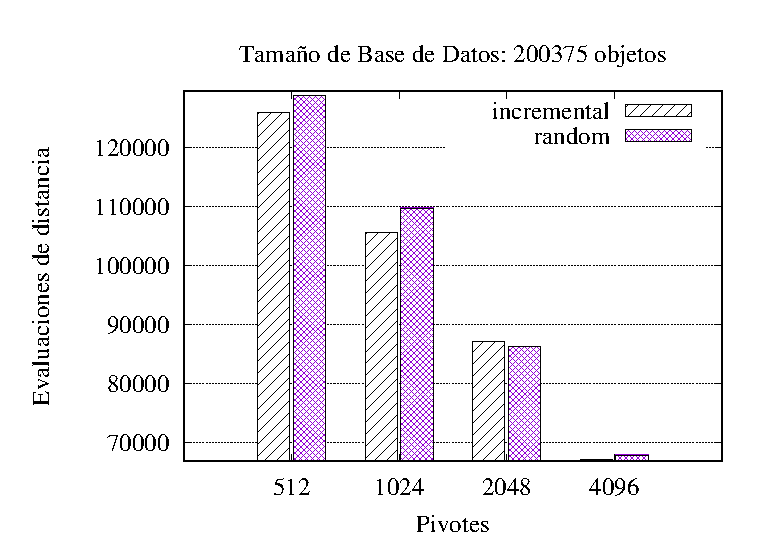
\includegraphics[width=71.5mm]{imagenes/random_vs_incremental/g4_200375.eps}}
{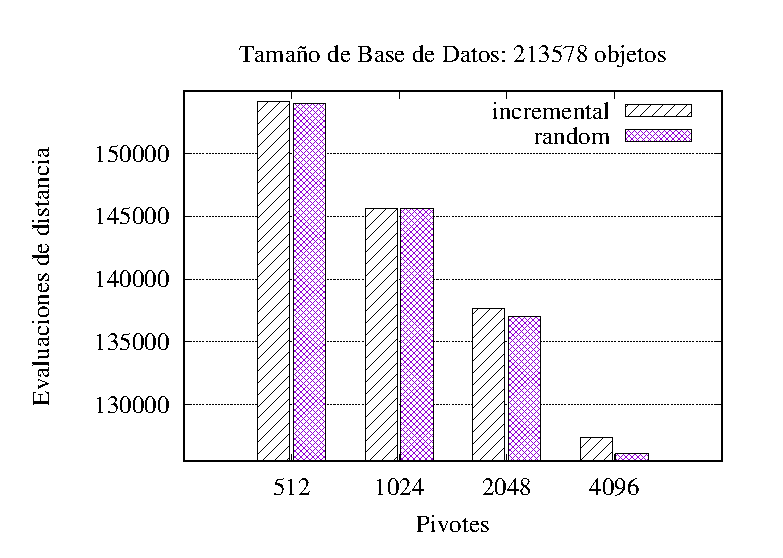
\includegraphics[width=71.5mm]{imagenes/random_vs_incremental/g4_213578.eps}}
\caption{\small Grupo 4 - Efecto de las t\'ecnicas de selecci\'on de pivotes random vs incremental respecto de evaluaciones de distancia.}
\end{figure}
\chapter{Anexo II: }
% Contenido del anexo II